% Informe técnico — Laboratorio 11 (MLOps). Compilar dos veces con pdflatex desde esta carpeta.
% Las figuras se leen de ../evidencias/lab11/ (evidencias reales) y de diagrama_pipeline.pdf (Graphviz).
\documentclass[11pt,a4paper]{article}
\usepackage[utf8]{inputenc}
\usepackage[T1]{fontenc}
\usepackage{lmodern}
\usepackage[spanish,es-noshorthands,es-tabla]{babel}
\usepackage[margin=2.3cm]{geometry}
\usepackage{graphicx}
\usepackage{booktabs}
\usepackage{tabularx}
\usepackage{array}
\usepackage{longtable}
\usepackage{float}
\usepackage{enumitem}
\usepackage{xcolor}
\usepackage{caption}
\usepackage{titlesec}
\usepackage{fancyhdr}
\usepackage[hidelinks]{hyperref}

\graphicspath{{./}{../evidencias/lab11/}}
\titleformat*{\section}{\large\bfseries\color{black}}
\titleformat*{\subsection}{\normalsize\bfseries\color{black}}
\captionsetup{font=small,labelfont=bf}
\setlist{itemsep=2pt,topsep=3pt}
\newcolumntype{L}{>{\raggedright\arraybackslash}X}
\newcommand{\cod}[1]{\texttt{\small #1}}
\pagestyle{fancy}\fancyhf{}
\lhead{\small Observatorio de Inteligencia Turística}\rhead{\small CC3066 — Laboratorio 11}
\cfoot{\small\thepage}
\renewcommand{\headrulewidth}{0.4pt}
\sloppy

\begin{document}

% ------------------------------------------------------------------ carátula
\begin{titlepage}
\centering
{\large UNIVERSIDAD DEL VALLE DE GUATEMALA\par}
\vspace{0.3cm}
Facultad de Ingeniería\par
Departamento de Ciencias de la Computación\par
\vspace{1.6cm}
CC3066 --- Data Science\par
Laboratorio 11 --- MLOps: pipeline reproducible, trazabilidad y despliegue\par
\vspace{1.2cm}
{\LARGE Observatorio de Inteligencia Turística\par}
\vspace{0.3cm}
{\large Informe técnico de verificación y entrega\par}
\vspace{1.6cm}
\begin{tabular}{ll}
Francisco Martinez & 23617\\
Jonathan Zacarias & 231104\\
Mario Rocha & 23501\\
Luis Pedro Lira & 23669\\
\end{tabular}\par
\vspace{0.4cm}
{\small Integrantes y carnés tomados de la carátula del informe del Laboratorio 10\\(\cod{reporte\_final\_lab10/Laboratorio\_10\_Documento\_Diseno\_Final.pdf}).\par}
\vfill
Repositorio: \url{https://github.com/Zacatac23/Laboratorio-_10_Dashboard.}\\
{\small (debe pasar a visibilidad privada; ver §13)\par}
\vspace{0.6cm}
Guatemala, 2 de noviembre de 2026\par
\end{titlepage}

% ------------------------------------------------------------------ resumen
\section*{Resumen ejecutivo}
El Observatorio publica una estimación mensual de viajeros a Guatemala (serie \cod{Total} y siete subseries) mediante un pipeline batch reproducible: valida las fuentes con seis controles de calidad, evalúa el procedimiento sin fuga temporal frente a un baseline en los mismos meses, aplica una regla de aceptación predefinida, registra cada ejecución en MLflow y solo entonces publica de forma atómica la versión que lee el tablero.

En la verificación final (2 de noviembre de 2026): la suite de 100 pruebas automatizadas pasó (99 PASS y 1 omitida sin Docker; 100 PASS con Docker); dos pares de ejecuciones completas en contenedor fueron idénticos (diferencia máxima 0.0 en 504 estimaciones); siete fallos controlados se detectaron sin alterar la versión aprobada; se restauró una versión anterior con verificación SHA-256; y Docker Compose funcionó desde una copia limpia del commit \cod{bced471} con persistencia de MLflow tras \cod{down}/\cod{up}. El modelo activo (Promedio Histórico Mensual) obtiene MAE 80{,}365.74 y RMSE 94{,}175.26 viajeros/mes en 63 meses (abril 2021–junio 2026), frente a 235{,}730.91 y 253{,}203.39 del baseline Seasonal Naive en los mismos meses.

Se encontraron y corrigieron tres defectos (filtración de la URI de MLflow entre corridas, \cod{-{}-allowed-hosts} con puerto fijo y denominador cero detectado fuera de QC-E) y un problema visual del tablero. La correspondencia con cada inciso del enunciado (1.1--8.4) está en \cod{docs/auditoria\_final\_lab11.md}. Quedan abiertos: commitear la corrección de QC-E, hacer privado el repositorio y entregar el almacén de MLflow por un medio autorizado. Un backtest complementario muestra que, a 12 meses, el baseline supera al modelo activo en 6 de 8 cortes; se documenta como riesgo sin modificar reglas a posteriori.

% ------------------------------------------------------------------ alcance
\section{Alcance}
\begin{table}[H]\centering\small
\caption{Alcance de la estimación (fuente: \cod{config/pipeline\_config.yaml}).}
\begin{tabularx}{\textwidth}{@{}lL@{}}\toprule
Variable & \cod{viajeros}: ingreso mensual a Guatemala; \cod{Total} y subseries \cod{Via\_Aérea}, \cod{Via\_Terrestre}, \cod{Via\_Marítima}, \cod{Tipo\_Turista}, \cod{Tipo\_Excursionista}, \cod{Tipo\_Cruceristas}, \cod{Tipo\_Viajero}\\
Unidad / agregación & viajeros/mes, no negativa; mensual (\cod{YYYY-MM-01})\\
Fuentes & \cod{series\_mensuales.csv} (serie, fecha, viajeros) para modelado; \cod{pais\_mensual.csv} y \cod{via\_frontera.csv} como contexto (QC no bloqueante y monitoreo)\\
Periodos & Ajuste 2009-01 a 2021-03 (147 meses); evaluación 2021-04 a 2026-06 (63 meses), sin exclusiones\\
Modelo & Promedio Histórico Mensual (activo); Seasonal Naive lag 12 (baseline); Holt-Winters aditivo (referencia)\\
Factor de reparto & Proporción de cada subserie sobre el Total en el periodo de ajuste (p.\,ej. \cod{Tipo\_Turista} 0.7408, \cod{Via\_Terrestre} 0.5904, \cod{Via\_Aérea} 0.3759)\\
Salida & \cod{data/estimaciones\_aprobadas.csv} + manifiesto JSON (SHA-256, \cod{run\_id}, métricas, periodo)\\
\bottomrule\end{tabularx}
\end{table}

% ------------------------------------------------------------------ diagrama
\section{Diagrama del pipeline}
La Figura~\ref{fig:pipeline} resume el flujo implementado en \cod{src/pipeline.py}: dos compuertas (calidad y aceptación), verificación de trazabilidad antes de cualquier publicación y estados finales explícitos con su código de salida.
\begin{figure}[H]\centering
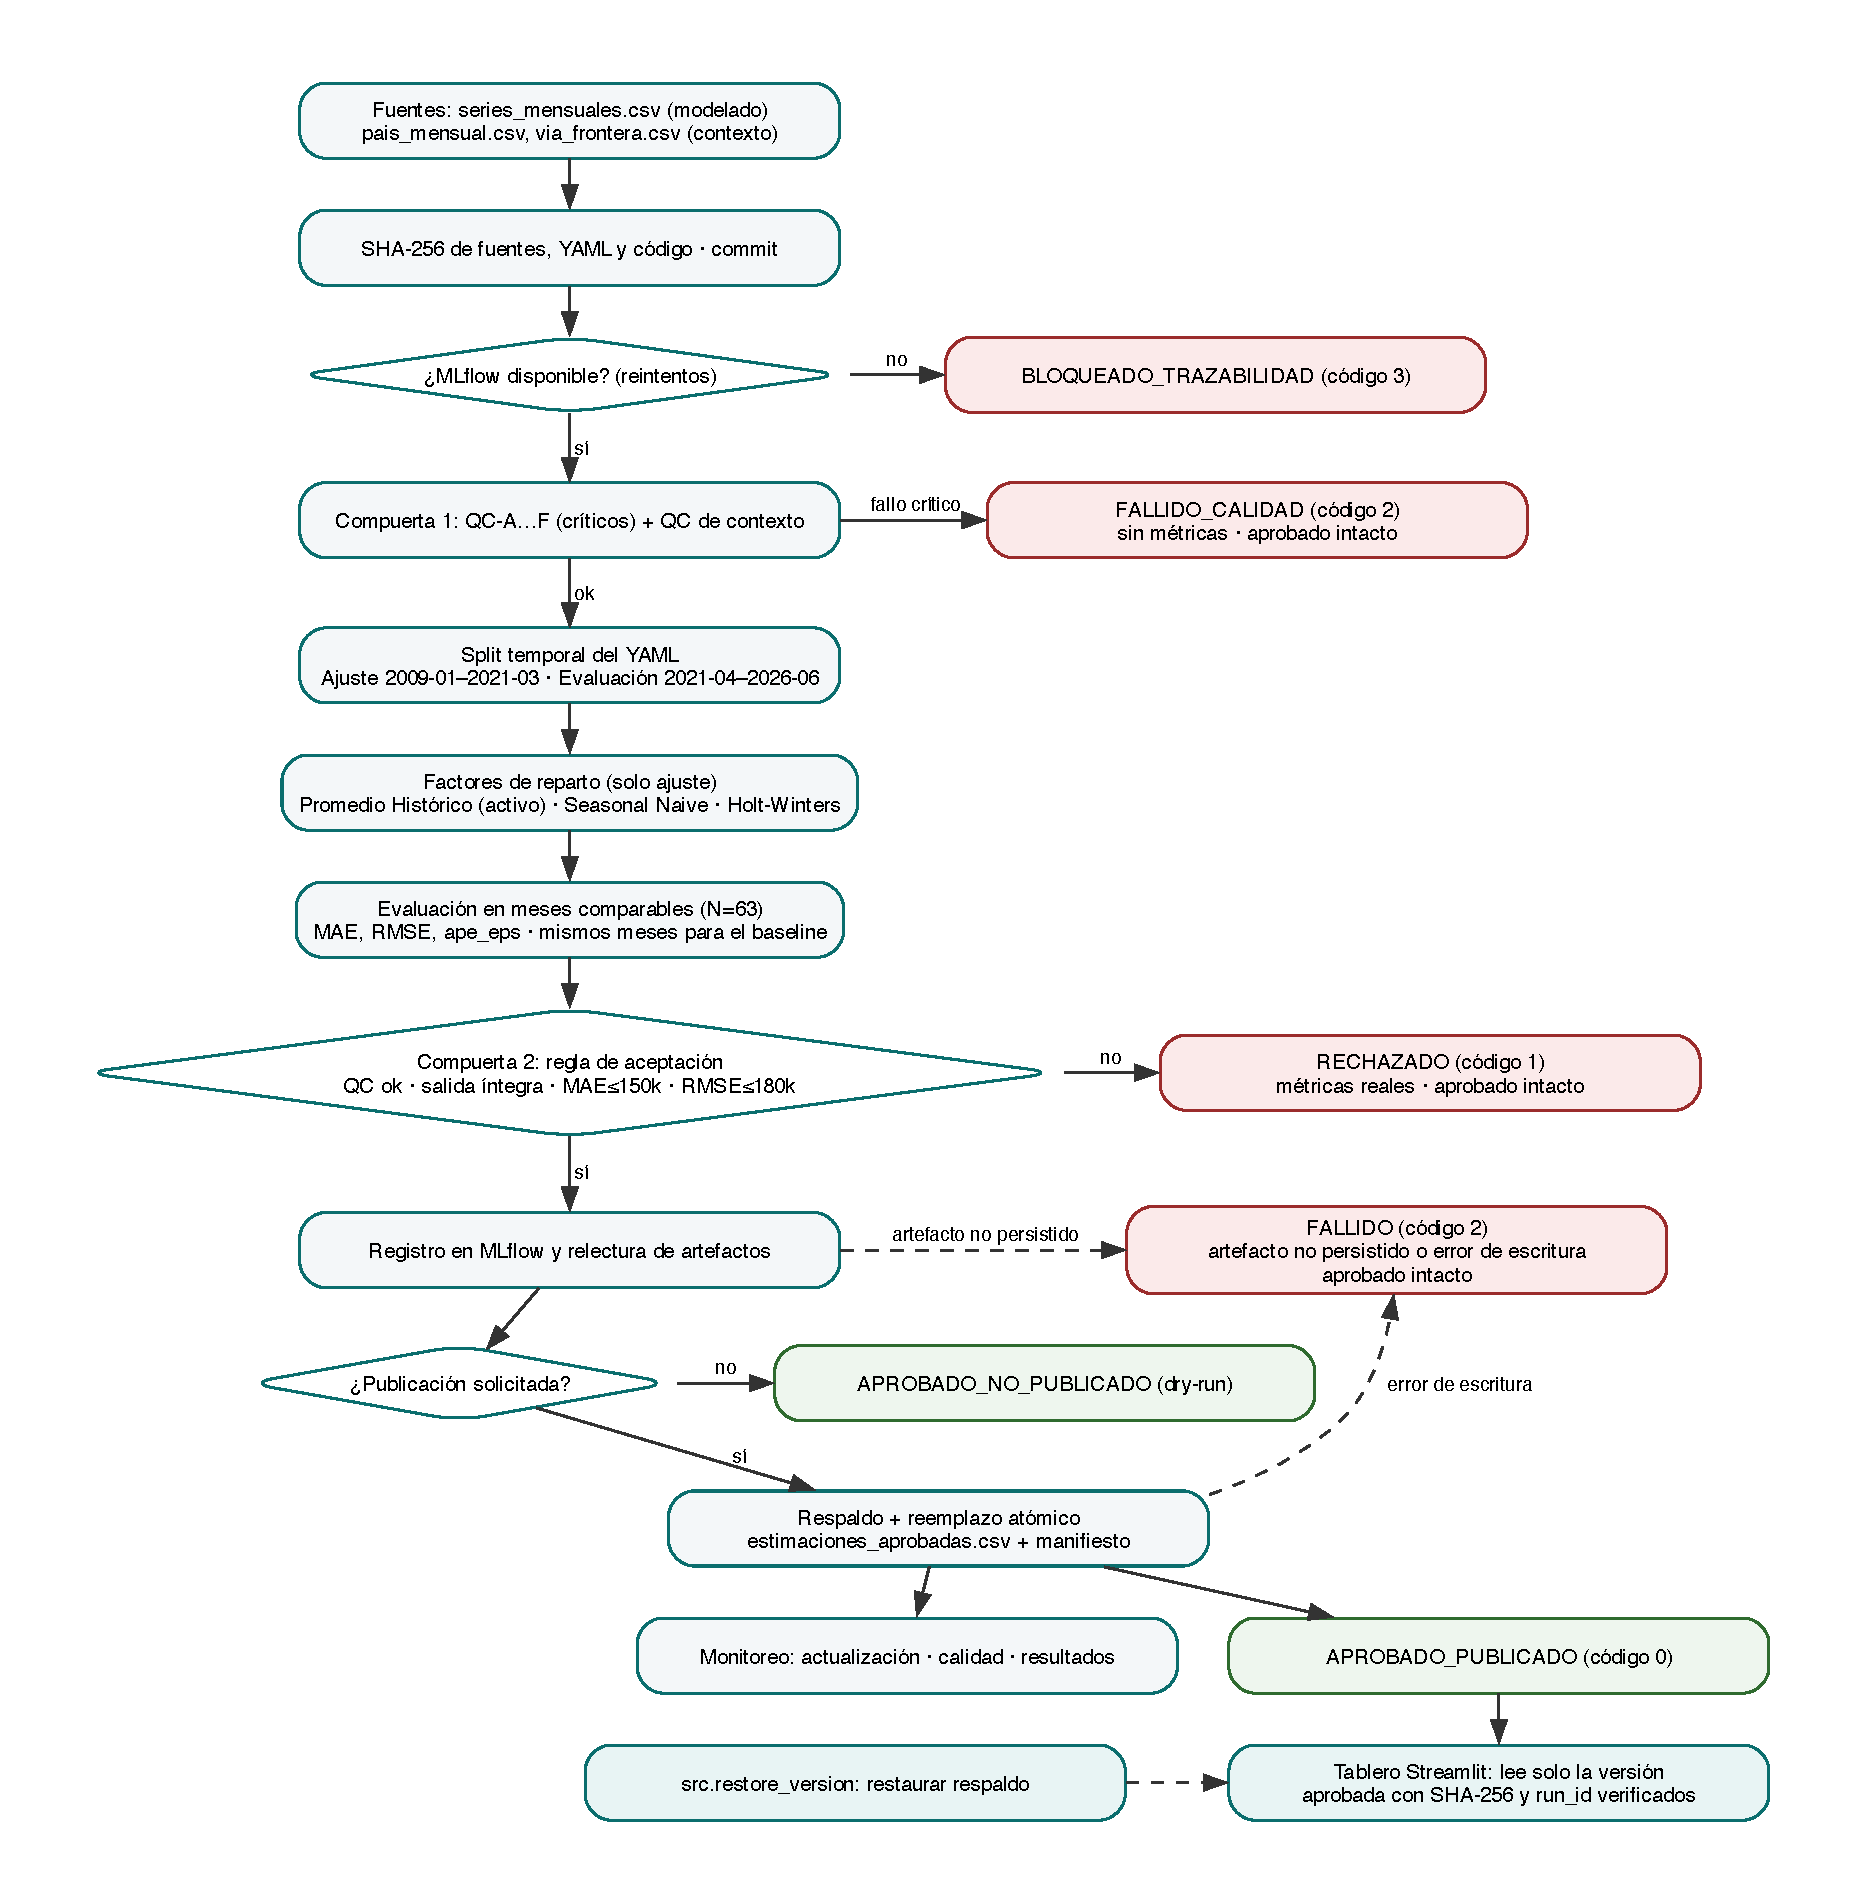
\includegraphics[width=0.86\textwidth]{diagrama_pipeline.pdf}
\caption{Pipeline real con puntos de validación, evaluación, aprobación, publicación y consulta. Fuente editable: \cod{reporte\_final\_lab11/diagrama\_pipeline.dot}.}
\label{fig:pipeline}
\end{figure}

% ------------------------------------------------------------------ preparación
\section{Preparación, ejecución reproducible y dependencias}
\begin{itemize}
\item Ejecución: \cod{python pipeline.py -{}-config config/pipeline\_config.yaml -{}-publish} o \cod{-{}-no-publish} (exactamente una). Códigos: 0 aprobado, 1 rechazado, 2 fallo, 3 bloqueado.
\item Configuración única en YAML: rutas, periodos, exclusiones, modelo activo, umbrales, semilla 42 y estrategia MLflow. Variables de entorno documentadas en \cod{.env.example}.
\item Dependencias: \cod{requirements.txt} (directas exactas) y \cod{requirements.lock}; imagen \cod{python:3.12.10-slim}. Entorno local verificado con Python 3.12.13 y \cod{pip check} sin conflictos.
\end{itemize}

% ------------------------------------------------------------------ QC
\section{Controles de calidad}
\begin{table}[H]\centering\small
\caption{Controles de \cod{src/quality\_checks.py} y resultado en las ejecuciones verificadas.}
\begin{tabularx}{\textwidth}{@{}lLL@{}}\toprule
Control & Detiene si\ldots & Resultado observado\\\midrule
QC-A Columnas y tipos & falta \cod{serie}/\cod{fecha}/\cod{viajeros} o tipo incompatible & PASSED con datos reales; FAILED al eliminar \cod{viajeros}\\
QC-B Fechas y cobertura & fecha inválida, día $\neq$ 1, hueco o ventana incompleta & PASSED (210 meses continuos)\\
QC-C Unicidad & clave (\cod{serie}, \cod{fecha}) duplicada & PASSED; FAILED al duplicar una fila\\
QC-D Faltantes & nulos en columnas indispensables & PASSED\\
QC-E Valores y denominadores & NaN, infinito o negativo (cero válido) o denominador del factor de reparto (suma del Total en ajuste) igual a 0 & PASSED; FAILED con Total 2015-03 = $-500$ y con el ajuste en 0\\
QC-F Regla metodológica & Total difiere $>$2\,\% de la suma de vías o faltan insumos & PASSED; FAILED/NO\_VERIFICABLE en los fallos inyectados\\
Contexto & duplicados/valores en \cod{pais\_mensual}, \cod{via\_frontera} & Advertencia, no bloqueo (prueba \cod{FuentesMultiples})\\
\bottomrule\end{tabularx}
\end{table}
\noindent\textbf{Denominador cero (inciso 3.1 e).} QC-E verifica el denominador del factor de reparto antes del modelado; con el periodo de ajuste en cero la corrida termina \cod{FALLIDO\_CALIDAD} (prueba \cod{DenominadorCeroEnQC}, que falla sin el cambio). Antes de este ajuste el caso solo se detectaba en el cálculo de factores (\cod{FALLIDO}, etapa de modelado); esa validación se conserva como segunda barrera. Cada control registra qué verifica, su estado (PASSED, WARNING, FAILED o NO\_VERIFICABLE) y si es crítico en \cod{reports/quality\_report\_<run>.json}; los periodos sin cobertura no se imputan con cero.

% ------------------------------------------------------------------ MLflow
\section{Trazabilidad con MLflow}
Cada run registra: estado, commit (en contenedor, declarado por \cod{GIT\_COMMIT}), SHA-256 de las tres fuentes, del YAML y del código, semilla, split, factores, perfil del modelo, reporte QC, regla y decisión, métricas del modelo y de los baselines, monitoreo, auditoría, estimaciones candidatas y manifiesto (11 artefactos, Figura~\ref{fig:mlflow}). Los artefactos se releen antes de publicar.

\begin{table}[H]\centering\small
\caption{Dos ejecuciones completas en el servidor MLflow de Docker Compose (\cod{reports/reproducibilidad\_lab11.json}).}\label{tab:repro}
\begin{tabularx}{\textwidth}{@{}llL@{}}\toprule
Run del pipeline & ID MLflow & Estado\\\midrule
\cod{run\_20261102\_001410\_ce7eea} & {\footnotesize\texttt{7787c39f59d64cf69394bde8de3ea709}} & aprobado, no publicado (dry-run)\\
\cod{run\_20261102\_001413\_338a6e} & {\footnotesize\texttt{575d18e094f245f1bf51697e3cd11381}} & aprobado, no publicado (dry-run)\\\midrule
\multicolumn{3}{@{}p{\dimexpr\textwidth}@{}}{Comparación: 8 series $\times$ 63 meses con \cod{np.allclose(atol=1e-6, rtol=0)}; diferencia máxima 0.0; \cod{config.sha256} (\cod{d12e42c6\ldots}), \cod{code.sha256} (\cod{54c04097\ldots}) y hashes de fuentes idénticos; 25 métricas idénticas. Estado: REPRODUCIBLE. Volátiles ignorados: \cod{run\_id}, tiempos, duración y columnas \cod{run\_id}/\cod{fecha\_generacion} del CSV candidato.}\\
\bottomrule\end{tabularx}
\end{table}

\begin{figure}[H]\centering
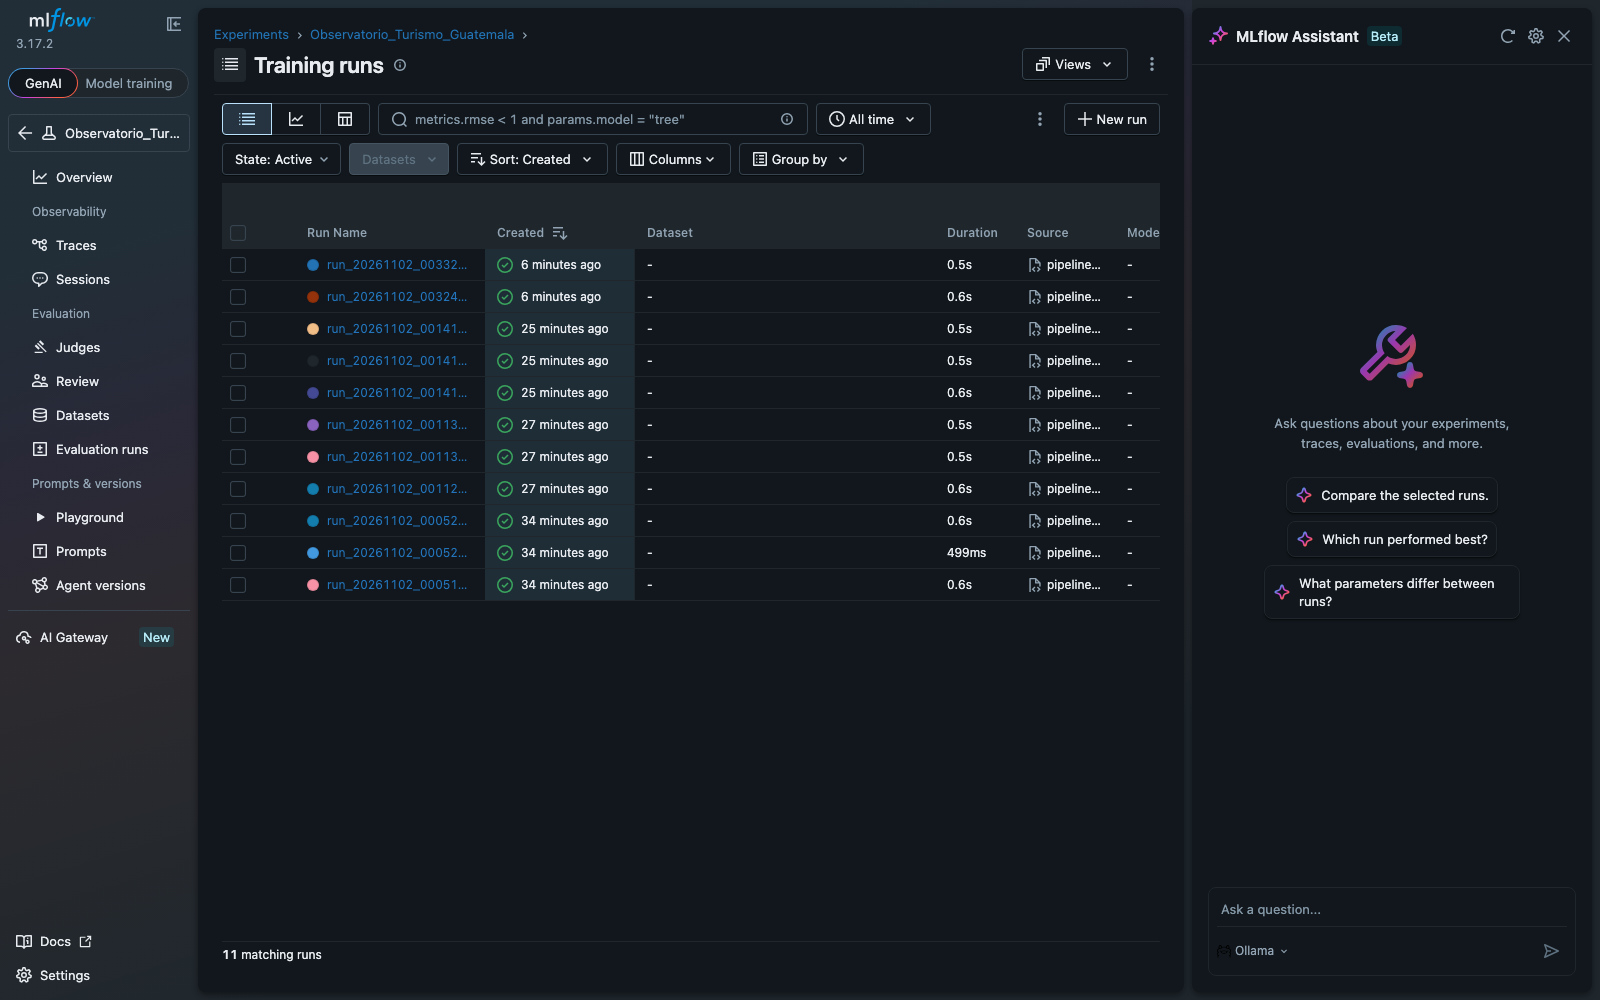
\includegraphics[width=0.49\textwidth]{mlflow/ui_01_experimento_runs.png}\hfill
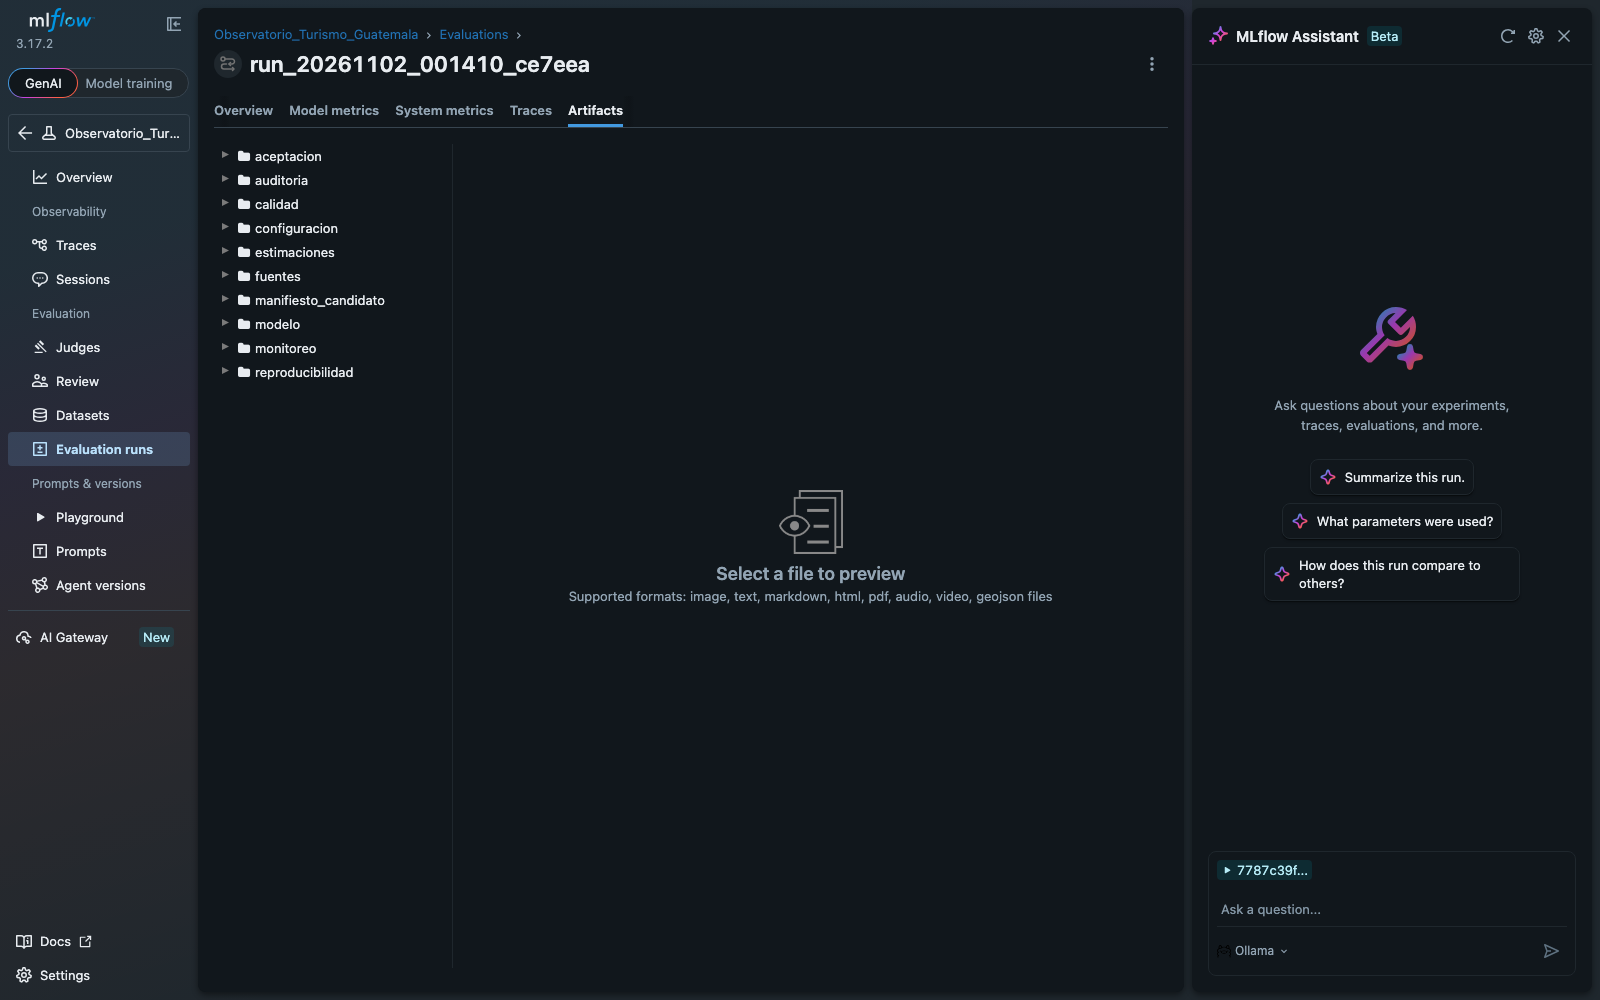
\includegraphics[width=0.49\textwidth]{mlflow/ui_04_run_artefactos.png}
\caption{UI real de MLflow en el servidor de Compose (puerto 5001 por conflicto con AirPlay en macOS). Izquierda: 9 runs del experimento \cod{Observatorio\_Turismo\_Guatemala}. Derecha: carpetas de artefactos del run \cod{run\_20261102\_001410\_ce7eea}.}
\label{fig:mlflow}
\end{figure}
\noindent Holt-Winters no es reproducible entre sistemas operativos (MAE 302{,}827.47 en Linux/Docker frente a 178{,}765.59 registrado en Windows en la etapa previa), por el optimizador numérico; no es el modelo activo. La exportación completa de runs está en \cod{evidencias/lab11/mlflow/export\_runs.json}.

% ------------------------------------------------------------------ evaluación
\section{Validación temporal}
Backtest de origen fijo: ajuste hasta 2021-03 y estimación de los 63 meses siguientes sin reajuste. Solo se evalúan meses con observación finita; enero y febrero de 2026 tienen dato y se evalúan (la memoria anterior decía lo contrario). La prueba \cod{SinFugaTemporal} demuestra que multiplicar por 10 los meses evaluados no cambia ningún parámetro, factor ni predicción. La métrica relativa es \cod{ape\_eps} $=\overline{|e|/(|y|+1)}\times 100$, no el MAPE convencional.

\begin{table}[H]\centering\small
\caption{Métricas en los mismos 63 meses (run \cod{run\_20261102\_001410\_ce7eea}).}
\begin{tabular}{@{}lrrrr@{}}\toprule
Procedimiento & MAE & RMSE & ape\_eps \% & N\\\midrule
Promedio Histórico Mensual (activo) & 80{,}365.74 & 94{,}175.26 & 38.67 & 63\\
Seasonal Naive lag 12 (baseline) & 235{,}730.91 & 253{,}203.39 & 83.86 & 63\\
Holt-Winters aditivo (referencia) & 302{,}827.47 & 327{,}720.16 & 103.99 & 63\\
\bottomrule\end{tabular}
\end{table}

\begin{table}[H]\centering\small
\caption{Backtest complementario de cortes múltiples (horizonte 12 meses, mismos meses por corte). Fuente: \cod{evidencias/lab11/evaluacion/backtest\_cortes\_multiples.json}.}
\begin{tabular}{@{}lrrr@{}}\toprule
Origen (evalúa los 12 meses siguientes) & Activo & Seasonal Naive & Holt-Winters\\\midrule
2016-12 & 113{,}813.60 & 42{,}363.00 & 29{,}482.86\\
2017-12 & 129{,}075.01 & 32{,}755.12 & 25{,}021.62\\
2018-12 & 152{,}456.80 & 42{,}261.10 & 22{,}247.41\\
2019-12 (evalúa 2020, COVID-19) & 211{,}364.21 & 306{,}100.68 & 328{,}357.30\\
2022-12 & 36{,}019.73 & 112{,}255.28 & 209{,}448.82\\
2023-12 & 58{,}299.74 & 36{,}983.58 & 21{,}869.34\\
2024-12 & 54{,}936.17 & 18{,}024.33 & 10{,}777.61\\
2025-06 & 48{,}607.14 & 12{,}237.42 & 14{,}590.48\\\midrule
MAE promedio & 100{,}571.55 & 75{,}372.56 & 82{,}724.43\\
\bottomrule\end{tabular}
\end{table}
\noindent A 12 meses el baseline supera al modelo activo en 6 de 8 cortes. El promedio histórico es robusto a la ruptura de 2020--2021 (gana en 2019-12 y 2022-12), pero desaprovecha la información reciente. No se modificó el modelo ni la regla después de observarlo; se recomienda evaluar el cambio de modelo en una versión futura con reglas fijadas de antemano.

\paragraph{Limitaciones de enero--febrero de 2026 (incisos 5.1 y 5.5).} Ambos meses tienen valor observado en la fuente mensual y coinciden en las tres fuentes institucionales (319{,}106 y 254{,}048 viajeros), por eso se evalúan. El backtest no reproduce la situación real de esos meses: (1) se estiman desde el origen fijo 2021-03, con horizonte de 58--59 meses, no con la información disponible a inicios de 2026; (2) la fuente no documenta si las cifras son preliminares o revisadas, así que su comparabilidad institucional no está certificada; (3) 2026 es parcial (hasta junio). Como análisis de sensibilidad, sin cambiar la regla (\cod{scripts/lab11/sensibilidad\_ene\_feb\_2026.py}), sin esos dos meses el MAE del modelo activo pasa de 80{,}365.74 (N=63) a 81{,}388.83 (N=61) y el del baseline de 235{,}730.91 a 236{,}852.07: la decisión no cambia. Si la institución los declarara no comparables, la exclusión se registra en el YAML con su motivo antes de evaluar una nueva versión.

% ------------------------------------------------------------------ aceptación
\section{Regla de aceptación}
Predefinida en el YAML y aplicada por \cod{evaluate\_acceptance\_rule}: (1) todos los QC críticos aprobados; (2) salida íntegra: todas las series, sin nulos, finita y no negativa; (3) MAE $\le$ 150{,}000 y (4) RMSE $\le$ 180{,}000 viajeros/mes. Superar al baseline se registra (\cod{acceptance.beats\_baseline}) pero no es obligatorio. Justificación de escala: el Total observado en el periodo evaluado promedia 276{,}685 viajeros/mes (mediana 279{,}790; rango 74{,}914--526{,}190); el umbral acota errores de alrededor de la mitad del nivel típico y rechazaría a Holt-Winters (302{,}827). El candidato activo resultó \textbf{aprobado}. El rechazo por desempeño se verifica con datos sintéticos (\cod{test\_corrida\_rechazada\_registra\_metricas\_reales\_sin\_publicar}): queda \cod{RECHAZADO}, con métricas reales y sin publicar.

% ------------------------------------------------------------------ tablero
\section{Integración con el tablero}
El tablero lee exclusivamente \cod{estimaciones\_aprobadas.csv} y su manifiesto (\cod{data\_logic.cargar\_version\_aprobada}); las métricas solo se muestran si SHA-256 y \cod{run\_id} coinciden. No hay caché: una publicación o restauración se ve al recargar.
\begin{figure}[H]\centering
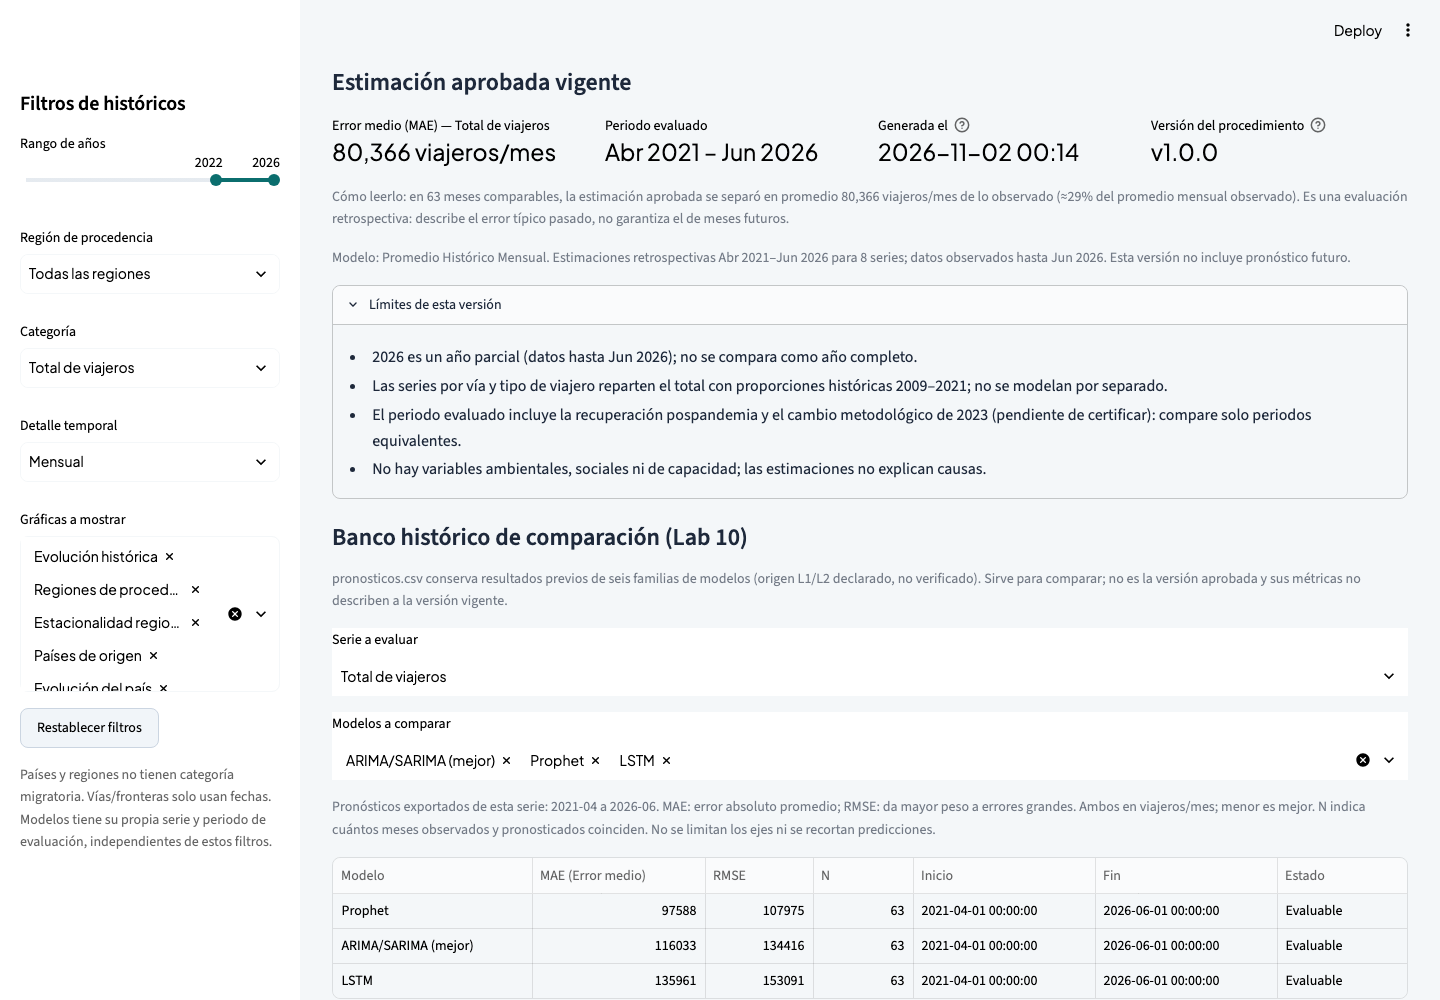
\includegraphics[width=0.49\textwidth]{dashboard/vigente_02_modelos_version_aprobada.png}\hfill
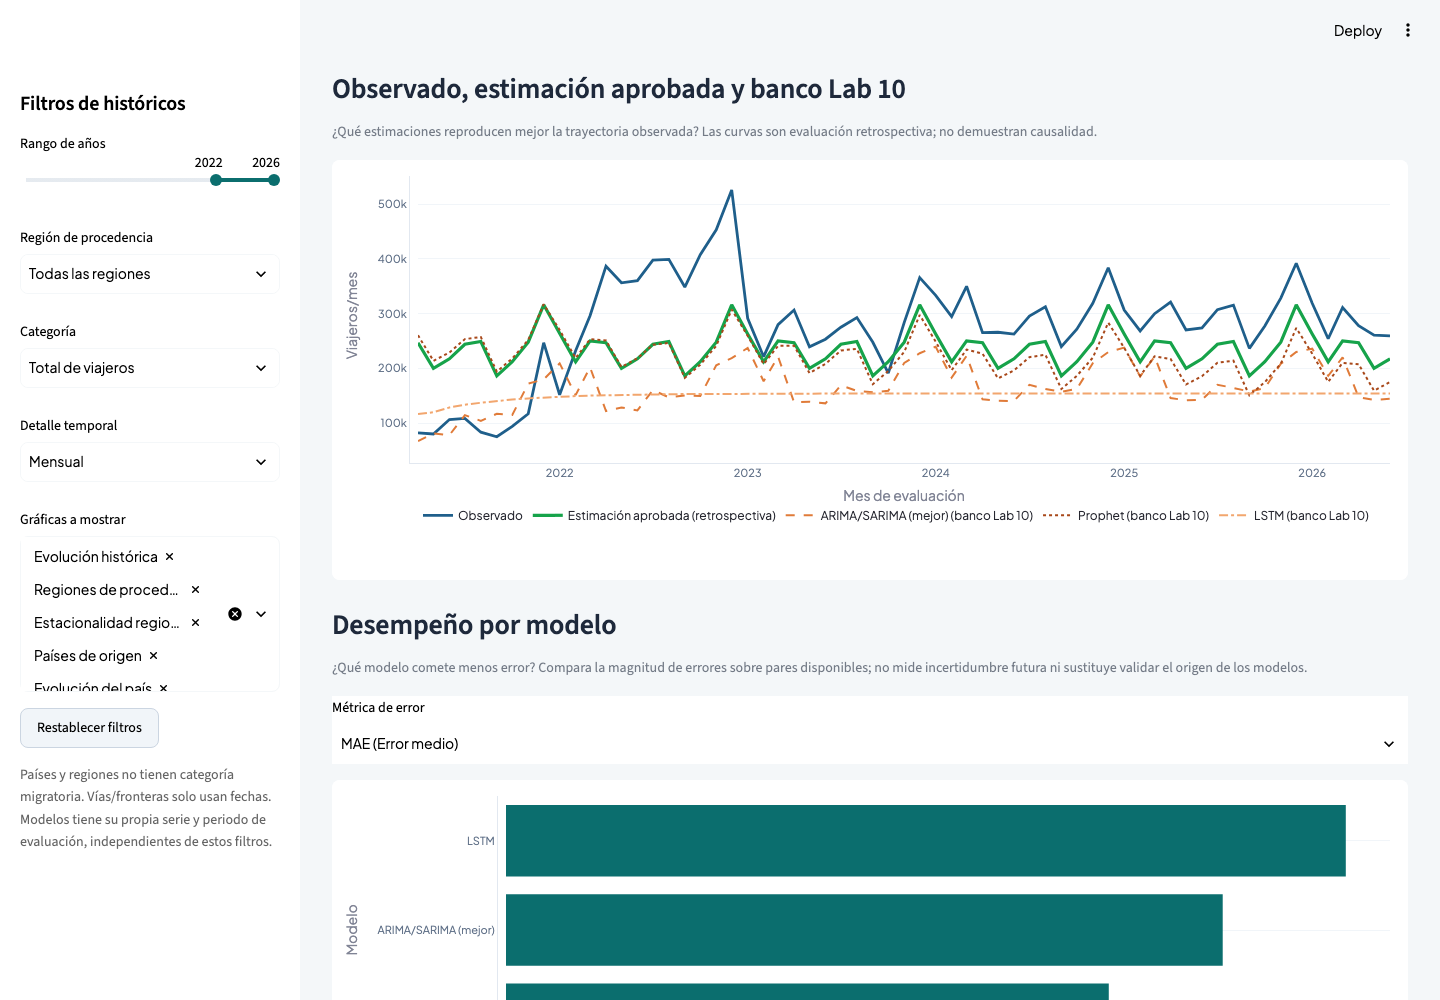
\includegraphics[width=0.49\textwidth]{dashboard/vigente_03_observado_vs_aprobada.png}
\caption{Tablero en Docker con la versión \cod{run\_20261102\_001416\_15b4a2}. Izquierda: MAE 80{,}366, periodo Abr 2021--Jun 2026, generada 2026-11-02 00:14, v1.0.0 y límites (2026 parcial, sin causalidad). Derecha: observado (azul), estimación aprobada (verde) y banco Lab 10 (discontinuas).}
\end{figure}
\begin{figure}[H]\centering
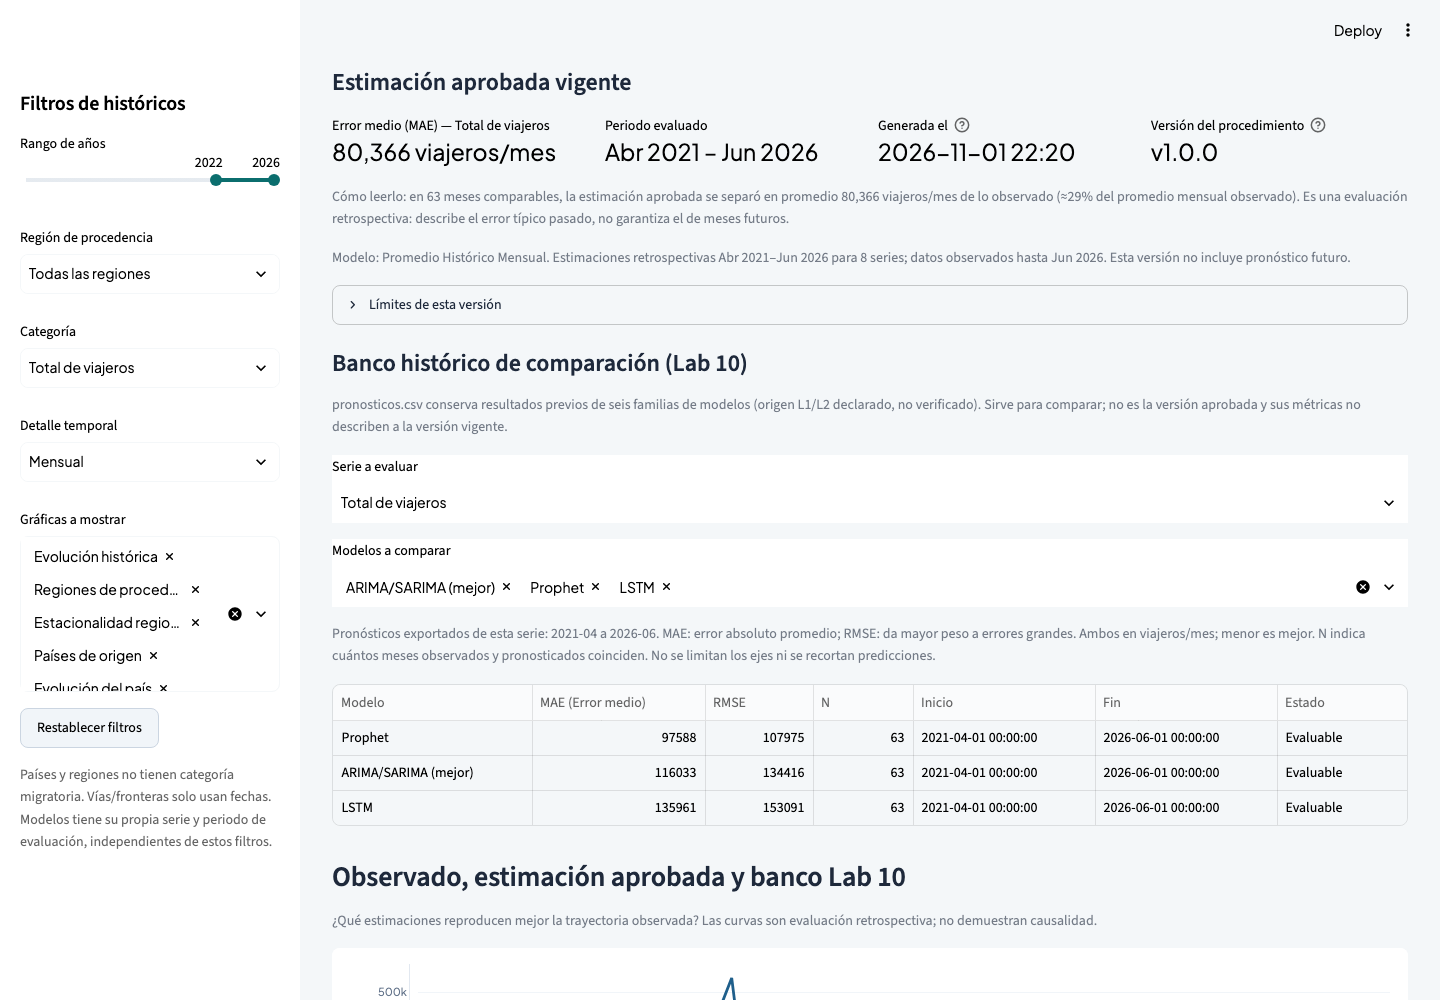
\includegraphics[width=0.49\textwidth]{dashboard/restaurada_01_modelos_version_restaurada.png}\hfill
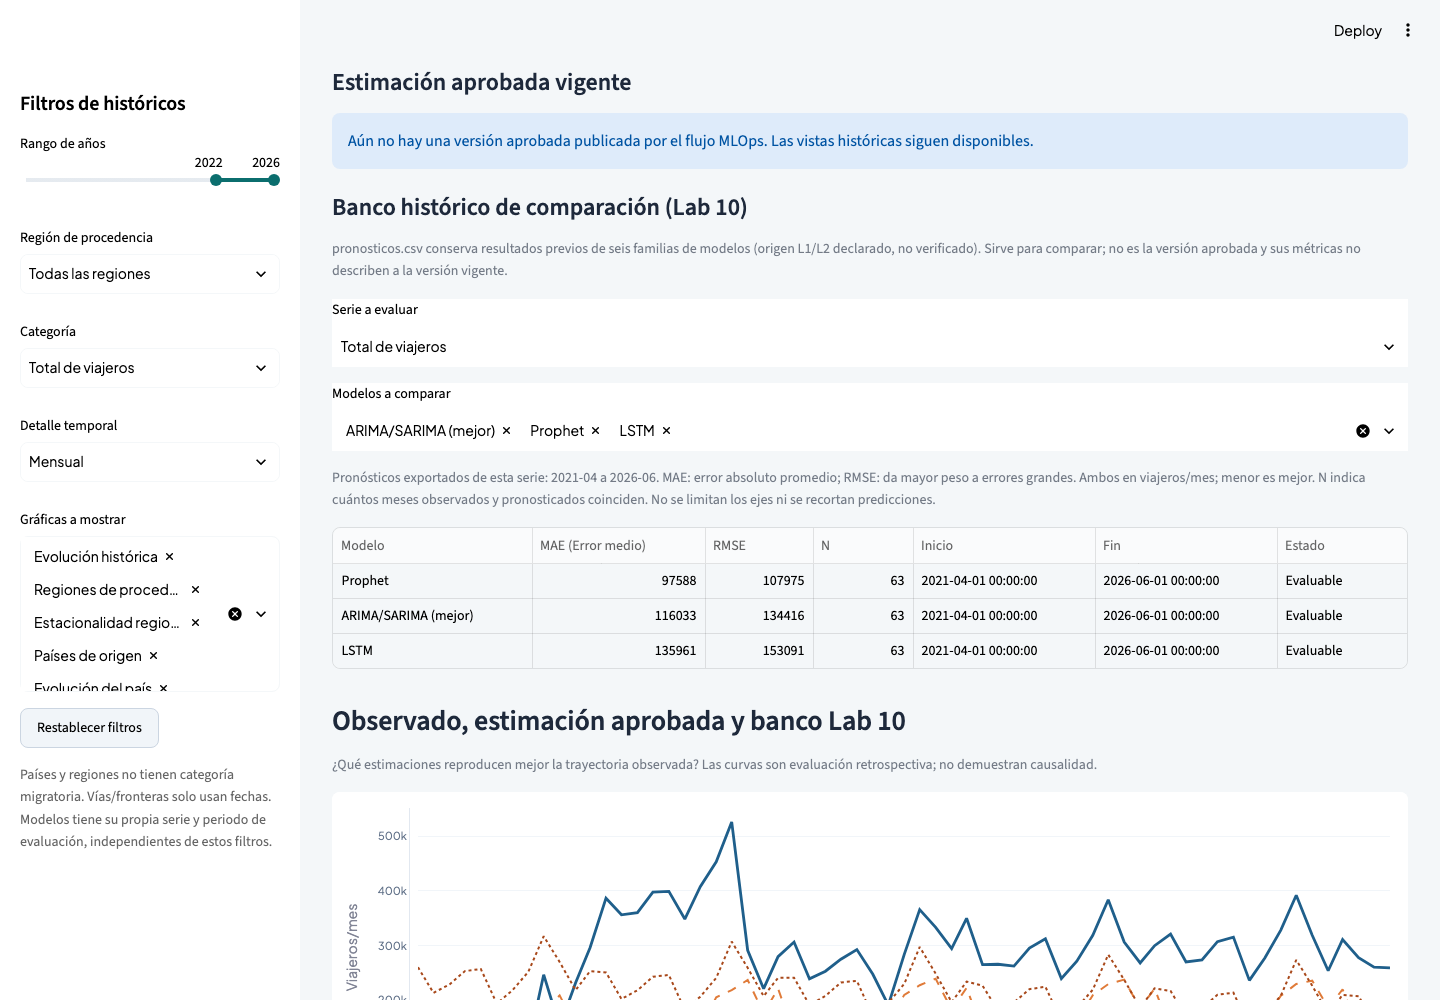
\includegraphics[width=0.49\textwidth]{dashboard/sin_aprobada_01_modelos_aviso.png}
\caption{Izquierda: tras restaurar el respaldo, el tablero muestra la versión \cod{run\_20261101\_222030\_d65c3b} (generada 2026-11-01 22:20). Derecha: sin archivo aprobado aparece un aviso informativo y las vistas históricas siguen disponibles.}
\end{figure}
\noindent Cambiar filtros (selector de vista, restablecer, cambio de pestañas) no creó runs (24 antes y después) ni archivos de salida (31). Captura móvil y metadatos de cada imagen: \cod{evidencias/lab11/dashboard/}. Se corrigió el truncado de los valores de las tarjetas (\cod{styles.css}).

% ------------------------------------------------------------------ monitoreo
\section{Monitoreo}
\begin{table}[H]\centering\small
\caption{Demostración de las tres clases de monitoreo. Fuente: \cod{evidencias/lab11/recuperacion/}\allowbreak\cod{fallos\_controlados.json}.}
\begin{tabularx}{\textwidth}{@{}lLL@{}}\toprule
Clase & Situación inducida (copia temporal) & Alerta real\\\midrule
Línea base & Datos vigentes & 0 alertas\\
Actualización & Serie truncada a 2026-04 (cobertura esperada 2026-06) & ALERTA: última observación 2026-04-01 no alcanza 2026-06\\
Calidad & 25 filas duplicadas frente a la ejecución previa & ALERTA: tasa de duplicados 0.0147 $>$ 0.0\\
Resultados & Total 2024-07 multiplicado por 3 & REVISIÓN: variación intermensual +236.8\,\% y $-$66.0\,\% ($>$50\,\%)\\
\bottomrule\end{tabularx}
\end{table}
\noindent El umbral de 50\,\% se justifica en el YAML: en 2009--2019 el percentil 95 de la variación intermensual del Total fue 32.4\,\%. Una alerta de variación pide revisión; no implica pérdida de precisión.

% ------------------------------------------------------------------ fallos
\section{Prueba controlada de falla, recuperación y restauración}
Sobre una copia temporal de \cod{data/} (versión aprobada inicial A: \cod{run\_20261101\_222030\_d65c3b}, SHA-256 \cod{d5795b8c\ldots}) se inyectó cada falla por separado:
\begin{table}[H]\centering\small
\caption{Fallos inyectados y contención (ejecuciones registradas en el experimento \cod{\ldots\_pruebas\_controladas}).}
\begin{tabularx}{\textwidth}{@{}LlLc@{}}\toprule
Falla & Estado & Detección & Aprobado intacto\\\midrule
Columna \cod{viajeros} ausente & FALLIDO\_CALIDAD & QC-A, QC-F & Sí\\
Clave duplicada & FALLIDO\_CALIDAD & QC-C, QC-F & Sí\\
Conteo negativo & FALLIDO\_CALIDAD & QC-E, QC-F & Sí\\
Denominador cero (ajuste en 0) & FALLIDO\_CALIDAD & QC-E (denominador del factor) & Sí\\
Error de escritura (\cod{os.replace}) & FALLIDO & publicación atómica; sin temporales & Sí\\
MLflow inaccesible & BLOQUEADO\_TRAZ. & verificación previa & Sí\\
Artefacto no persistido & FALLIDO & registro verificado & Sí\\
\bottomrule\end{tabularx}
\end{table}
Corregidos los datos, la recuperación publicó la versión B (\cod{run\_20261102\_013359\_237d8b}, \cod{59c2176b\ldots}). La restauración del respaldo de A con \cod{src.restore\_version} devolvió exactamente \cod{d5795b8c\ldots} y su manifiesto, y el tablero leyó A con metadatos verificados. En Docker se repitió la restauración con el CLI (\cod{restauracion\_docker.log}): el hash pasó de \cod{f201419b\ldots} a \cod{d5795b8c\ldots}, con respaldo de seguridad \cod{\_prerestauracion} y registro en \cod{logs/restore\_audit.jsonl}.

\paragraph{Defecto encontrado.} En la primera corrida de esta prueba, «MLflow inaccesible» terminó \cod{APROBADO\_PUBLICADO}: \cod{mlflow.set\_tracking\_uri()} escribe \cod{MLFLOW\_TRACKING\_URI} en el entorno y esa variable tiene prioridad sobre el YAML, de modo que una segunda corrida en el mismo proceso ignoraba su configuración. Se corrigió en \cod{TourismMLOpsPipeline.run()} y se agregó una prueba de regresión que falla sin la corrección.

% ------------------------------------------------------------------ docker
\section{Docker}
Servicios: \cod{mlflow} (SQLite y artefactos en el volumen \cod{observatorio\_turismo\_mlflow\_store}, \cod{-{}-serve-artifacts}, healthcheck), \cod{dashboard} (monta \cod{data/} en solo lectura) y \cod{pipeline} (perfil \cod{tools}). Imagen única \cod{observatorio-turismo:lab11} (1.61\,GB), usuario sin privilegios (uid 1000), puertos solo en 127.0.0.1.

Verificación desde copia limpia (inciso 8.4; \cod{docker\_verificacion.sh}, log en \cod{evidencias/lab11/docker/}): \cod{git clone} del commit \cod{bced471} sin archivos locales añadidos, 28 pasos con código 0. Incluye la inspección de la imagen (sin CSV, \cod{.db}, \cod{.env}, claves ni \cod{.git}; \cod{/app/data} vacío; uid 1000), \cod{up -d -{}-wait}, HTTP 200 en tablero y MLflow, dos dry-run en contenedor (\cod{run\_20261102\_013222\_08ad93} y \cod{run\_20261102\_013225\_d69796}, reproducibles con diferencia máxima 0.0 según \cod{reproducibilidad\_commit\_bced471.json}), una publicación (\cod{run\_20261102\_013228\_107c2c}) con respaldo de la versión anterior, y \cod{down}/\cod{up} sin \cod{-v} con los mismos 16 runs antes y después. El \cod{code.sha256} de esas corridas (\cod{54c04097\ldots}) es idéntico al de las corridas de la Tabla~\ref{tab:repro}, hechas antes del commit: el código registrado coincide con el versionado. La prueba automatizada \cod{DockerCompose} también pasó. Se corrigió \cod{-{}-allowed-hosts}, que fijaba el puerto 5000 e impedía usar la UI con otro puerto. \textbf{Advertencia:} \cod{docker compose down -v} borra el almacén de MLflow.

% ------------------------------------------------------------------ cierre
\section{Pruebas automatizadas}
\begin{table}[H]\centering\small
\caption{Resultados de \cod{python -B -m unittest discover -s tests -v}. La prueba omitida sin Docker es la de Compose, que requiere \cod{RUN\_DOCKER\_TESTS=1}. Fuente: \cod{evidencias/lab11/tests\_unitarios*.txt}.}
\begin{tabular}{@{}lrrrr@{}}\toprule
Corrida & Pruebas & PASS & FAIL & SKIP\\\midrule
Sin Docker & 100 & 99 & 0 & 1\\
Con Docker (\cod{MLFLOW\_PORT=5001}) & 100 & 100 & 0 & 0\\
\bottomrule\end{tabular}
\end{table}

\section{Limitaciones, riesgos y pendientes}
\begin{itemize}
\item \textbf{Commit:} la corrección de QC-E (inciso 3.1 e) y su prueba están sin commitear; la verificación desde copia limpia corresponde al commit \cod{bced471}. Tras commitear debe repetirse \cod{docker\_verificacion.sh}.
\item \textbf{Privacidad:} los repositorios remotos son públicos y los CSV institucionales están versionados; el enunciado exige un repositorio privado con acceso a docentes y auxiliares. El cambio de visibilidad corresponde al dueño.
\item \textbf{Registros de MLflow:} el almacén completo vive en el volumen Docker; se versiona solo la exportación JSON de runs. El volumen debe entregarse por un medio autorizado.
\item \textbf{Metodología:} a 12 meses el baseline supera al modelo activo en la mayoría de cortes; el umbral de MAE es tolerante (54\,\% del promedio observado); el reparto proporcional fija la estructura 2009--2021; el cambio metodológico de 2023 no está certificado.
\item \textbf{Operación:} restauraciones auditadas en local, no en MLflow; Holt-Winters dependiente del entorno.
\end{itemize}

\section{Conclusiones}
El flujo cumple su propósito de gobernanza: ninguna de las siete fallas probadas alteró la versión aprobada ni produjo una salida sin trazabilidad, las ejecuciones son reproducibles bit a bit dentro del mismo entorno, MLflow conserva los registros tras recrear contenedores y el tablero comunica la versión vigente con su error, su fecha y sus límites. La principal mejora pendiente es metodológica (revisar el modelo activo con reglas fijadas de antemano) y administrativa (repositorio privado y entrega autorizada de los registros de MLflow).

\section*{Referencias a evidencias}
Todas las rutas son relativas al repositorio: \cod{docs/guia\_evidencias\_lab11.md} (índice), \cod{evidencias/lab11/} (tests, Docker, MLflow, evaluación, recuperación y tablero), \cod{reports/reproducibilidad\_lab11.json}, \cod{docs/auditoria\_final\_lab11.md} y \cod{docs/resumen\_entrega\_lab11.md}.

\end{document}
